\documentclass{beamer}
\usepackage{hyperref}
\usetheme{Madrid}
\title{Coarse graining molecular dynamics with graph neural networks}
\author{Andrew Bruce\inst{1}}
\institute[UCSC] {
  \inst{1}
  University Of California, Santa Cruz
}
\date{2024-10-24}
\begin{document}
\frame{\titlepage}
\begin{frame}
  \frametitle{Problem}
  \href{https://arxiv.org/abs/1706.08566}{First paper link}
  \begin{block}{Why}
    Evaluating the forces on atoms in a protein is very computationally expensive.
  \end{block}
  Create some ``model'' that takes in $n$ atom types $\mathbf{Z} = ( Z_1, \dots, Z_n)$ and positions $\mathbf{R} = ( \vec{r}_1, \dots, \vec{r}_n )$, where $ \vec{r}_i \in \mathbb{R}^3$ and tries to calculate the forces $\mathbf{\hat{F}}(\mathbf{R}, \mathbf{Z}) = ( \vec{f}_1, \dots, \vec{f}_n )$ on each atom. It should be \alert{invariant} over translations and rotations. The force field should preserve the conservation of energy. The model should also be able to take in \alert{any number} of atoms.
\end{frame}
\begin{frame}
  \frametitle{Enforcing Invariants}
  \begin{block}{Rotations and translations}
    Make the model only use the distances between atoms, \alert{NOT} their absolute cartesian coordinates.
  \end{block}
  The model should only depend on $\| \vec{r}_i - \vec{r}_j \|$ between any two atoms, but \alert{never} $\vec{r}_i$ alone.
\end{frame}
\begin{frame}
  \frametitle{Enforcing Invariants}
  \begin{block}{Conservation of energy}
    Instead of the model calculating the forces $\mathbf{\hat{F}}(\mathbf{R}, \mathbf{Z}) \in \mathbb{R}^{3 \times n}$, calculate the energy $E(\mathbf{R}, \mathbf{Z}) \in \mathbb{R}$, then take the \alert{gradient with respect to the positions} to calculate the force.
    $\mathbf{\hat{F}} = \nabla_{\mathbf{R}} E$
  \end{block}
  Any force field like this is now impossible: 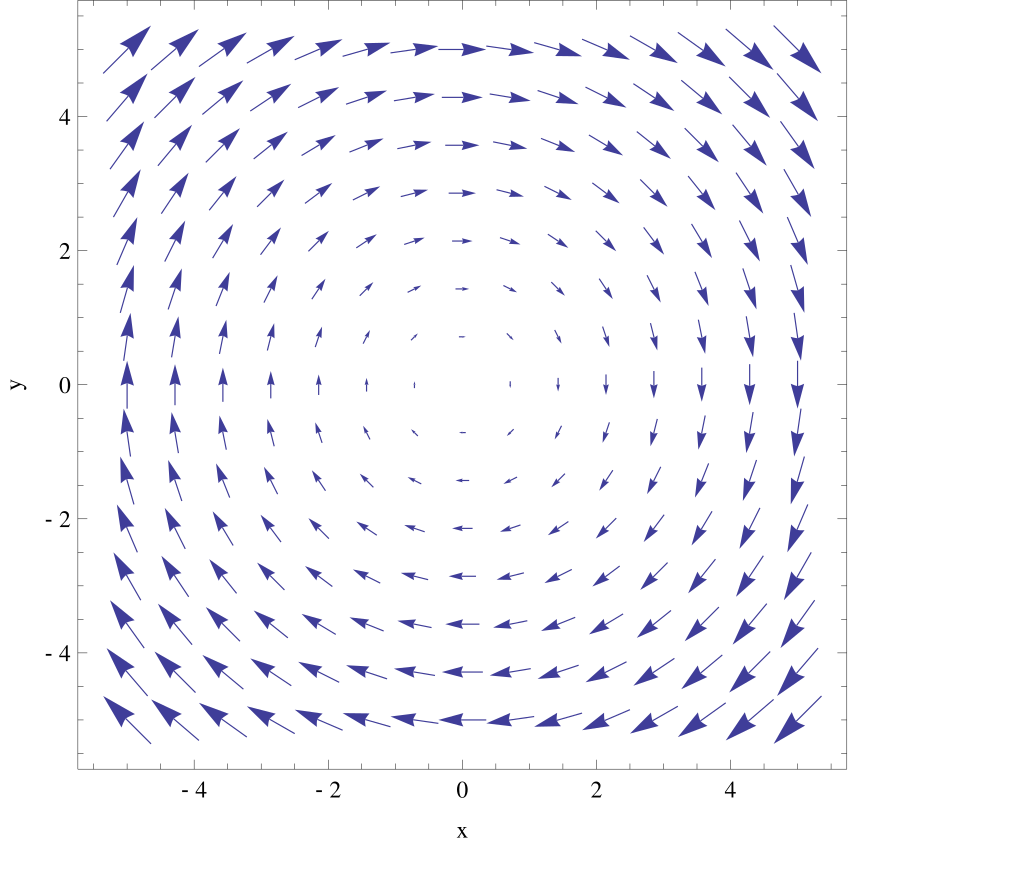
\includegraphics[width=0.35\linewidth]{./curl.png}
\end{frame}
\begin{frame}
  \frametitle{Schnet Architecture}
  \begin{center}
    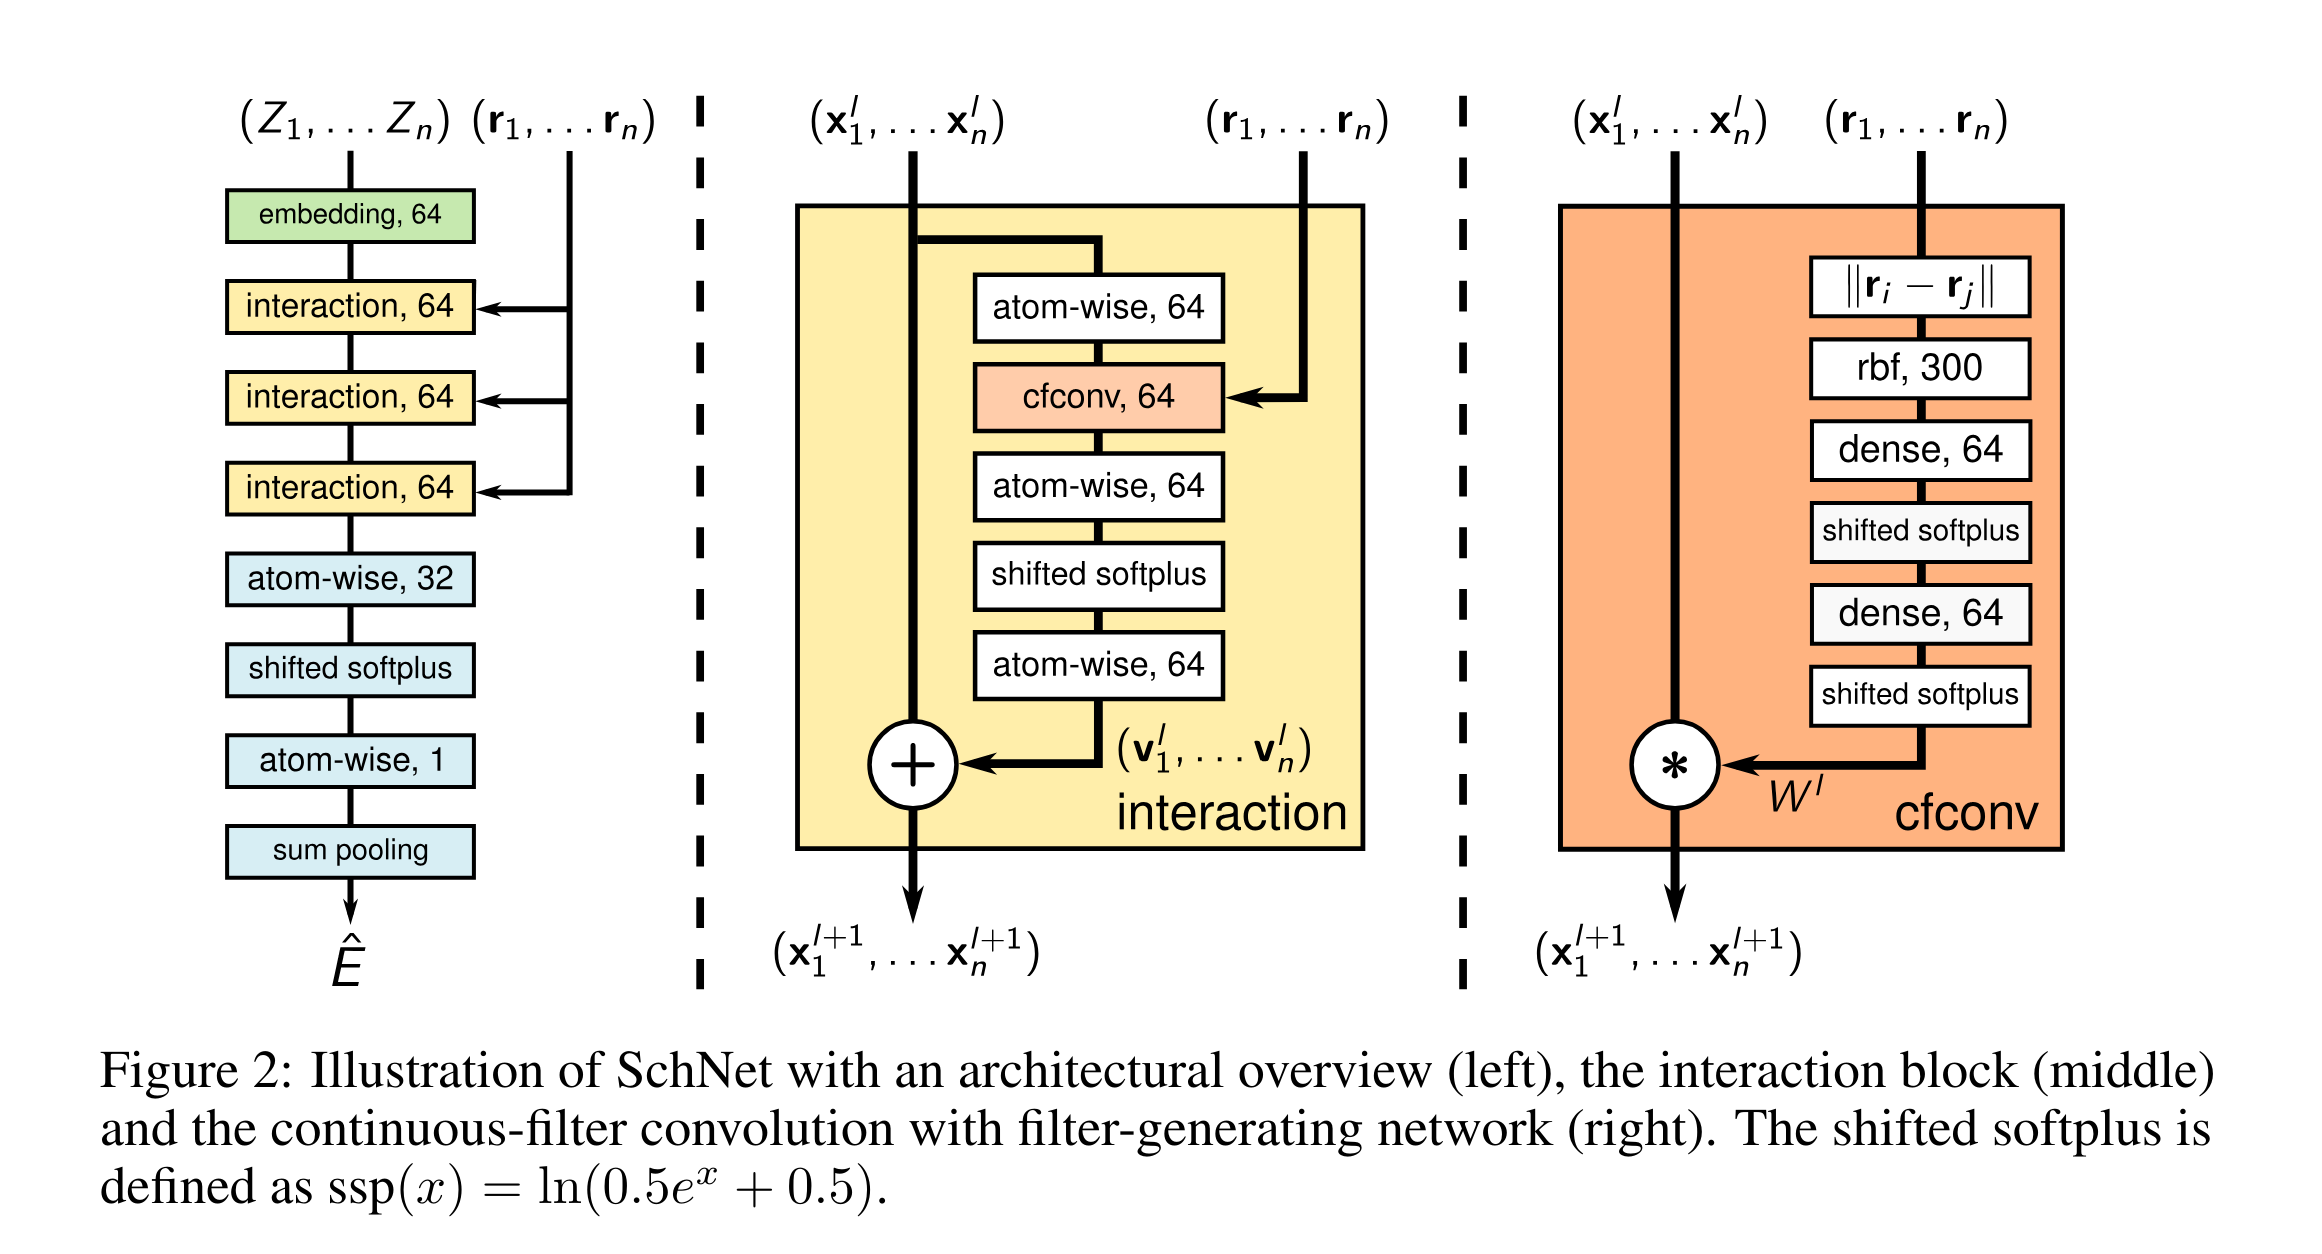
\includegraphics[width=0.5\linewidth]{./archetecture_overview.png}
  \end{center}
  The input embeddings are based off the atom type, $\vec{x}^0_i = a_{Z_i}$.
  \begin{block}{Atom wise layers}
    For each atom wise layer The parameters $W$ an $b$ are applied to the features of each atom $i$.
    $$\vec{x}_i^{l+1} = W\vec{x}_i^l + b$$
  \end{block}
\end{frame}
\begin{frame}
  \frametitle{Continuous-filter convolutions}
  \begin{minipage}{4cm}
    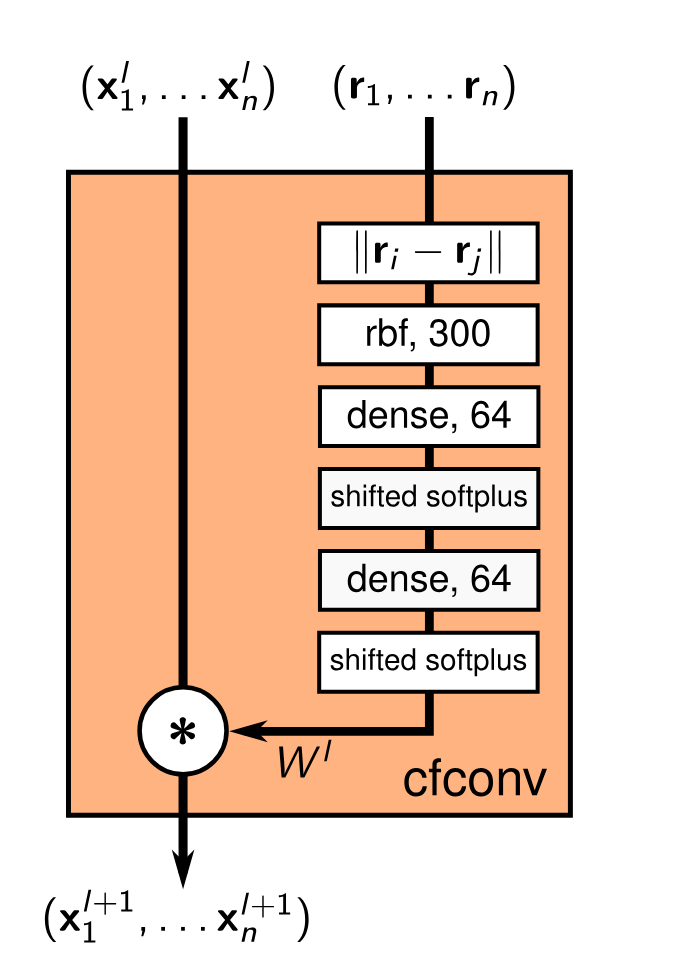
\includegraphics[width=\linewidth]{./cfconv_block.png}
  \end{minipage}% needs this comment for linebreak or something?
  \small\begin{minipage}{8cm}
  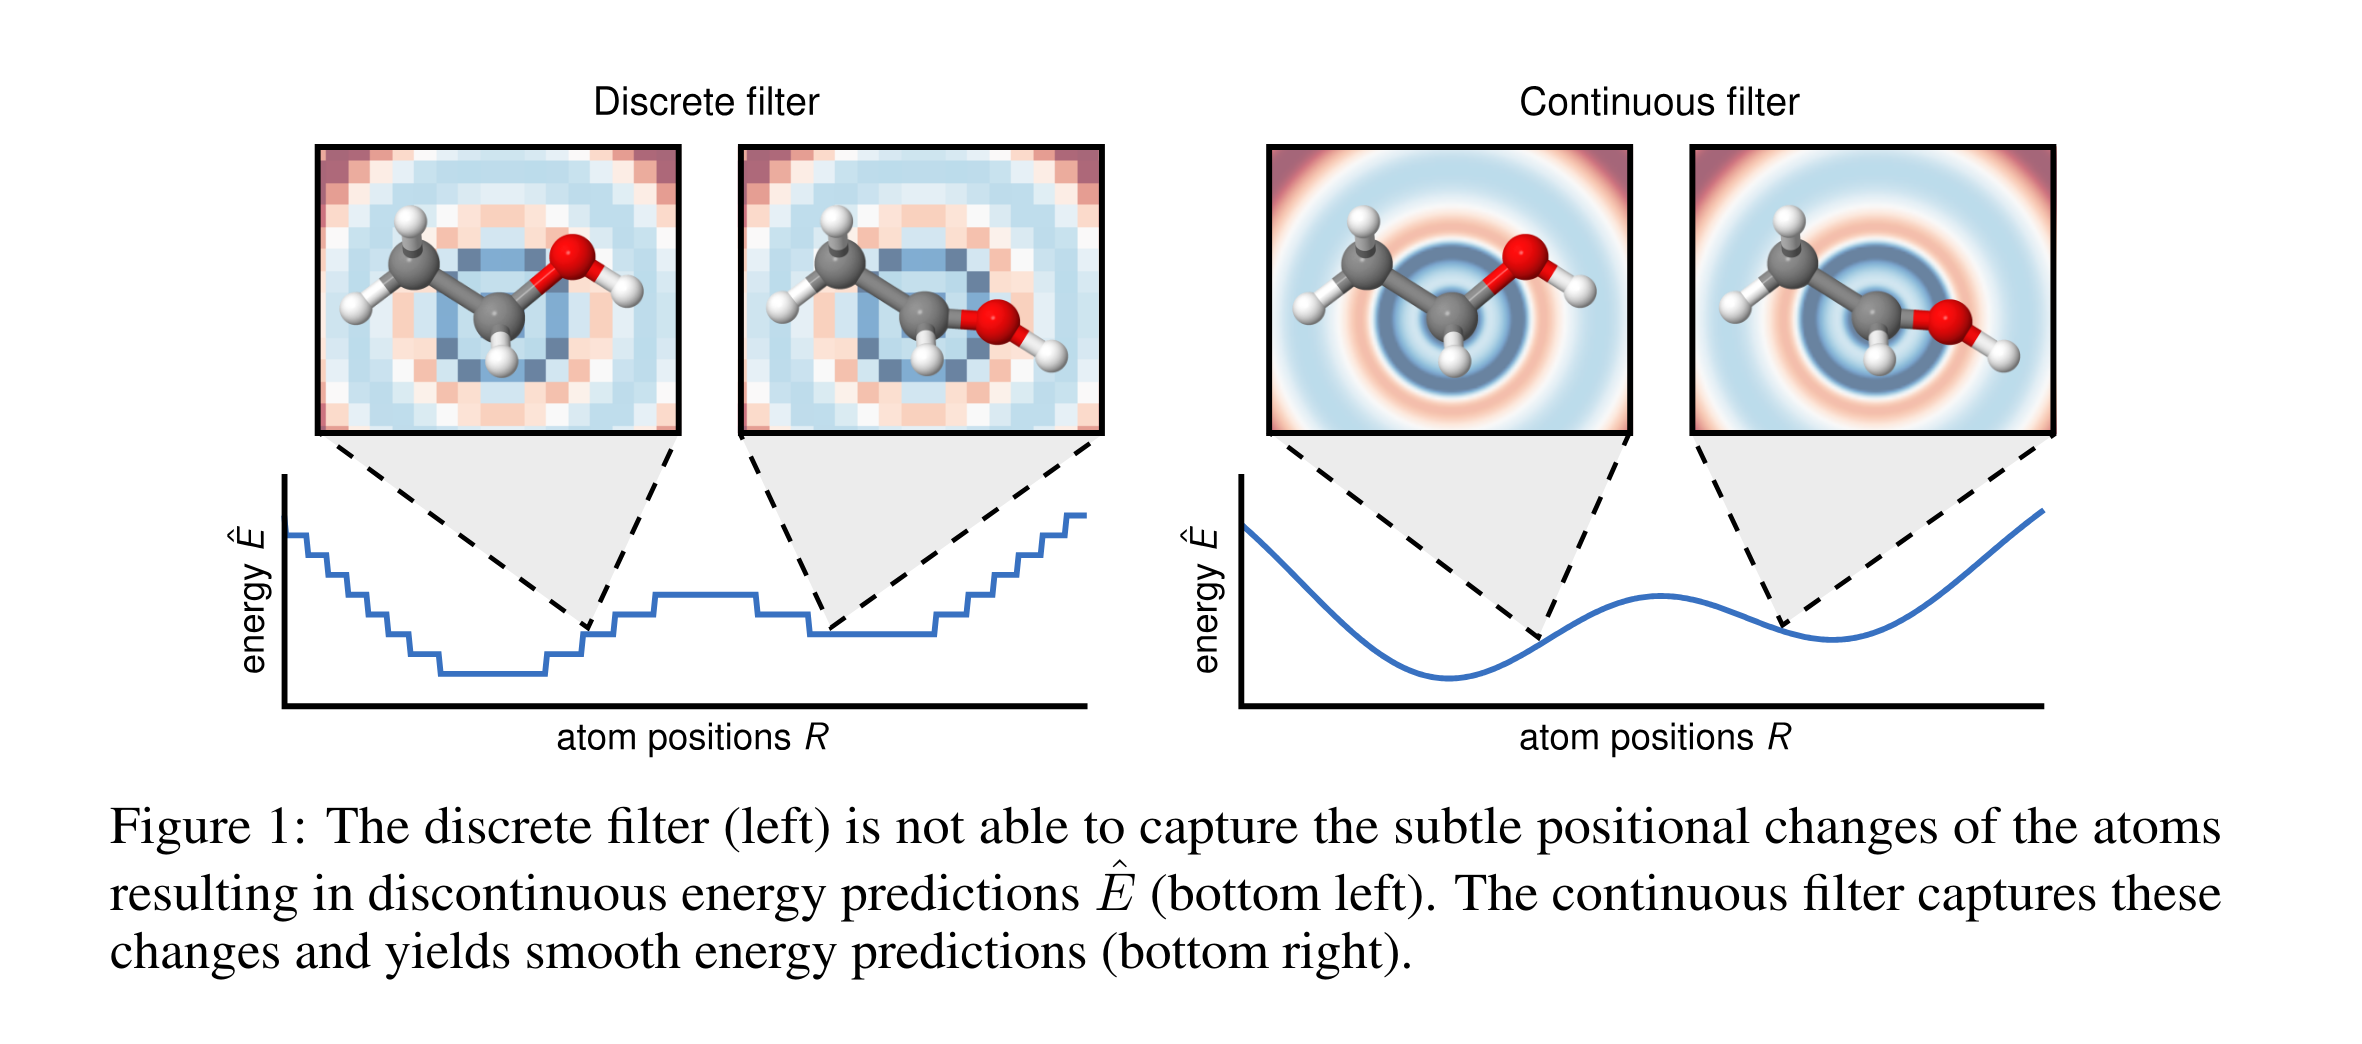
\includegraphics[width=\linewidth]{./cfconv.png}
  Attempt continious convolutions for unevenly spaced points.
  Learn some filter function $W$, and for each atom $i$ the next feature is $\vec{x}_i^{l+1} = \sum_j \vec{x}_j^l \circ W(\vec{r}_i - \vec{r}_j)$, where $\circ$ is element wise multiplication.
  \end{minipage}
  \begin{block}{Radial basis function}
    The radial basis functions will create a vector $\vec{e}$ where each element $\vec{e}_k(\vec{r}_i - \vec{r}_j) = e^{-\gamma (||r_i - r_j|| - \mu_k)^2}$.
  \end{block}
\end{frame}
\begin{frame}
  \frametitle{Training}
  The loss function is a combined energy and force loss. The output of the model $M$ is just one scalar, the energy $E = M(\mathbf{Z}, \mathbf{R})$. Given the training data consisting of the real energy $E^{real}$ and forces $F^{real}$.
  \begin{center}
    $L(M, \mathbf{Z}, \mathbf{R}) = \text{energy error} + \text{force error}$\\
    $= \rho(M(\mathbf{Z}, \mathbf{R}) - E^{real})^2 + \dfrac{1}{n} \| F^{real} - \nabla_{\mathbf{R}}M(\mathbf{Z}, \mathbf{R}) \|^2$\\
    $= \rho(E - E^{real})^2 + \dfrac{1}{n} \sum^n_{i=1} \sum^3_{d=1} ( F^{real}_{i_d} - \dfrac{\partial E}{\partial r_{i_d}} )^2$
  \end{center}
  \begin{block}{Double differentiation? Double backpropigation?}
    Gradient descent with respect to the weights $\mathbf{W}$ is:
    \begin{center}
      $\mathbf{W}_{t+1} = \mathbf{W}_t - \lambda \nabla_{\mathbf{W}} L(W)$
    \end{center}
    The entire network must be double differentiable...
  \end{block}
\end{frame}
\begin{frame}
  \frametitle{Results}
  Not that good ... but the invention of the continious-filter convolution will be useful in the next paper.
  \begin{center}
    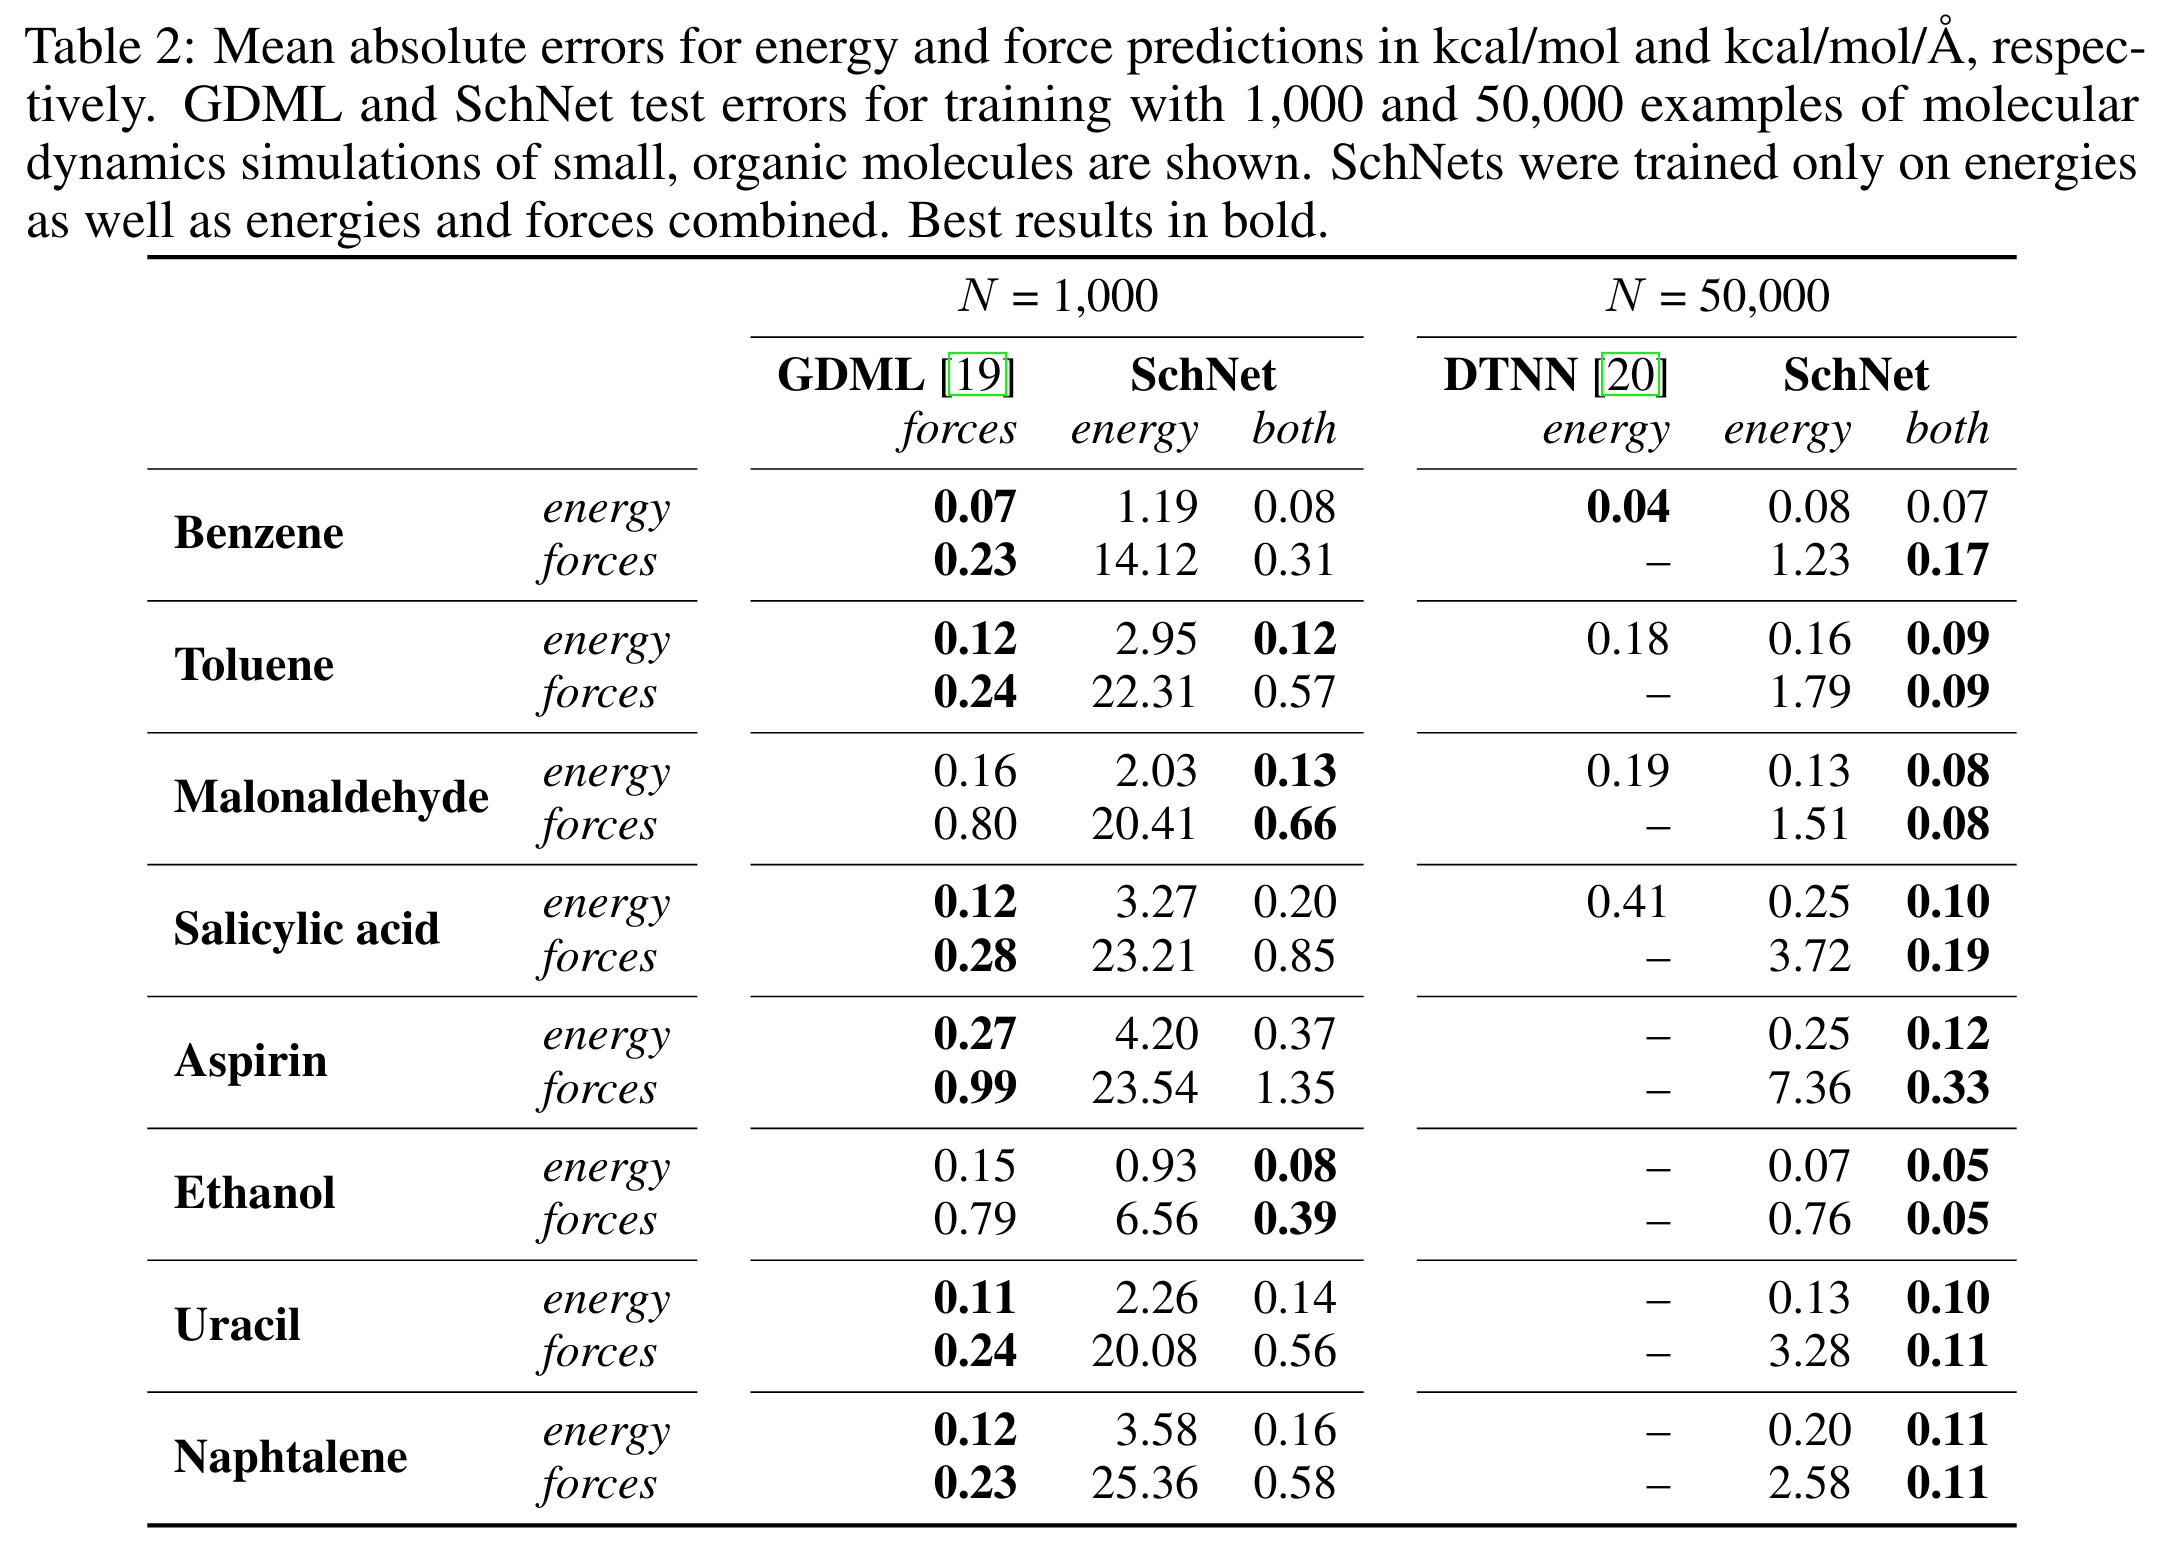
\includegraphics[width=0.7\linewidth]{./paper1_results.png}
  \end{center}
\end{frame}
\begin{frame}
  \frametitle{Paper 2}
  \huge \href{https://arxiv.org/abs/2007.11412}{Next paper link}\\
  \huge Schnet + CGNet = CGSchnet
\end{frame}
\begin{frame}
  \frametitle{Coarse graining}
  We want to map $N$ atoms to $n$ ``interaction sites''.
  We use a matrix $\Xi$ to map $\mathbb{R}^{3N} \longrightarrow \mathbb{R}^{3n}$. Given $R \in \mathbb{R}^{3N}$, the coarse grained $r = \Xi R$. Each interaction site is a linear combination of atom positions. (Also each row of $\Xi$ should sum to 1, so translations of all the atoms result in the the interaction sites being translated too.)
\end{frame}

\end{document}
